\documentclass[12pt,a4paper]{article}
\usepackage{fullpage}
\usepackage[top=2cm, bottom=4.5cm, left=2.5cm, right=2.5cm]{geometry}
\usepackage{amsmath,amsthm,amsfonts,amssymb,amscd}
\usepackage{lastpage}
\usepackage{enumitem}
\usepackage{fancyhdr}
\usepackage{mathrsfs}
\usepackage{xcolor}
\usepackage{graphicx}
\usepackage{listings}
\usepackage{hyperref}
\usepackage{tikz}
\usetikzlibrary{shapes,backgrounds}
\usepackage[utf8]{inputenc}
\usepackage[ruled, vlined]{algorithm2e}
% \usepackage{apacite}
\usepackage{csquotes}

% Edit these as appropriate
\newcommand\course{Reinforcement Learning}
\newcommand\NetID{sliu1@uvm.edu}
\newcommand\Author{Sida Liu}
\pagestyle{fancyplain}
\headheight 35pt
\lhead{\NetID\\\Author}
% \chead{\textbf{\Large Assignment \chapternumber }}
\rhead{\course \\ \today}
\lfoot{}
\cfoot{}
\rfoot{\small\thepage}
\headsep 1.5em

\setlength{\parskip}{\baselineskip}%
\setlength{\parindent}{0pt}%

\newenvironment{list_abc}
{ \begin{enumerate}[label=(\alph*)] }
{ \end{enumerate} }

\newenvironment{list_iv}
{ \begin{enumerate}[label=\roman*.] }
{ \end{enumerate} }

\hypersetup{
    colorlinks=true,
    linkcolor=blue,
    filecolor=magenta,      
    urlcolor=cyan,
}

\usepackage{tcolorbox}
\usepackage{booktabs}


\begin{document}

\section*{Revised Project Proposal}

\subsection*{Structure}
The deliverable will be a piece of open-source software.

\subsection*{Topic}

\subsubsection*{Motivation}
In 2017, Yoshua Bengio submitted an arXiv article named \emph{The Consciousness Prior} \cite{bengio_consciousness_2019}. 
He proposed the \emph{Consciousness Prior Theory}, which is about how, in his opinion, the \emph{Consciousness} works and how to implement the \emph{Global Workspace Theory} using recently developed \emph{Deep Learning} technology.
There are two major parts in his theory, the \emph{Consciousness} $c$ and the \emph{Unconsciousness} $h$.

I will focus on the $h$ in this course project because it is more practical and is the foundation before we get anything similar to the \emph{Consciousness}.

\subsubsection*{Big Picture of Deep Reinforcement Learning}
Our objective is to get a good $h$, but how can we get it.

Deep Learning is trying to do hierarchical information abstraction since its invention. 
CNN, RNN, Attention model, and many other Deep Learning models are very good tools to do this job.

In the setting of Reinforcement Learning, we can simply situate the agent in an environment, and use a high-level reward function to specify the goal.

At each time step, we can pass observation through the neural network model of the agent and get a value of that state (or action);
we can also use the Temporal Difference (TD) method to get a value of that state (or action).
We assume the TD method gives us the right value, so we adjust the parameters of the neural network model of the agent to make two values consistent.

This consistency is what we usually use to train an agent in Deep Reinforcement Learning.

\subsubsection*{Additional signal beside TD method}
What if the TD method doesn't give us the perfect value function? Do we have other sources of learning signals?

One possible learning signal can come from temporal consistency.
For example, we have two observations of two consecutive time steps.
We can assume the world doesn't change much in one single step, so the meaning of those two observations should be similar.
So we can pass two observations through the neural network model and compare two values produced.
They should be consistent.
And we can train the neural network model based on this consistency.

This might be an additional source for learning besides the TD method. 
I mention this because I think this is interesting, but it might not be quite related to my course project.

\subsubsection*{Course Project Plan}

I am planning to do Deep Reinforcement Learning.

I am not sure what the final project will look like, but I'll start the project with this:

\begin{figure}[h]
    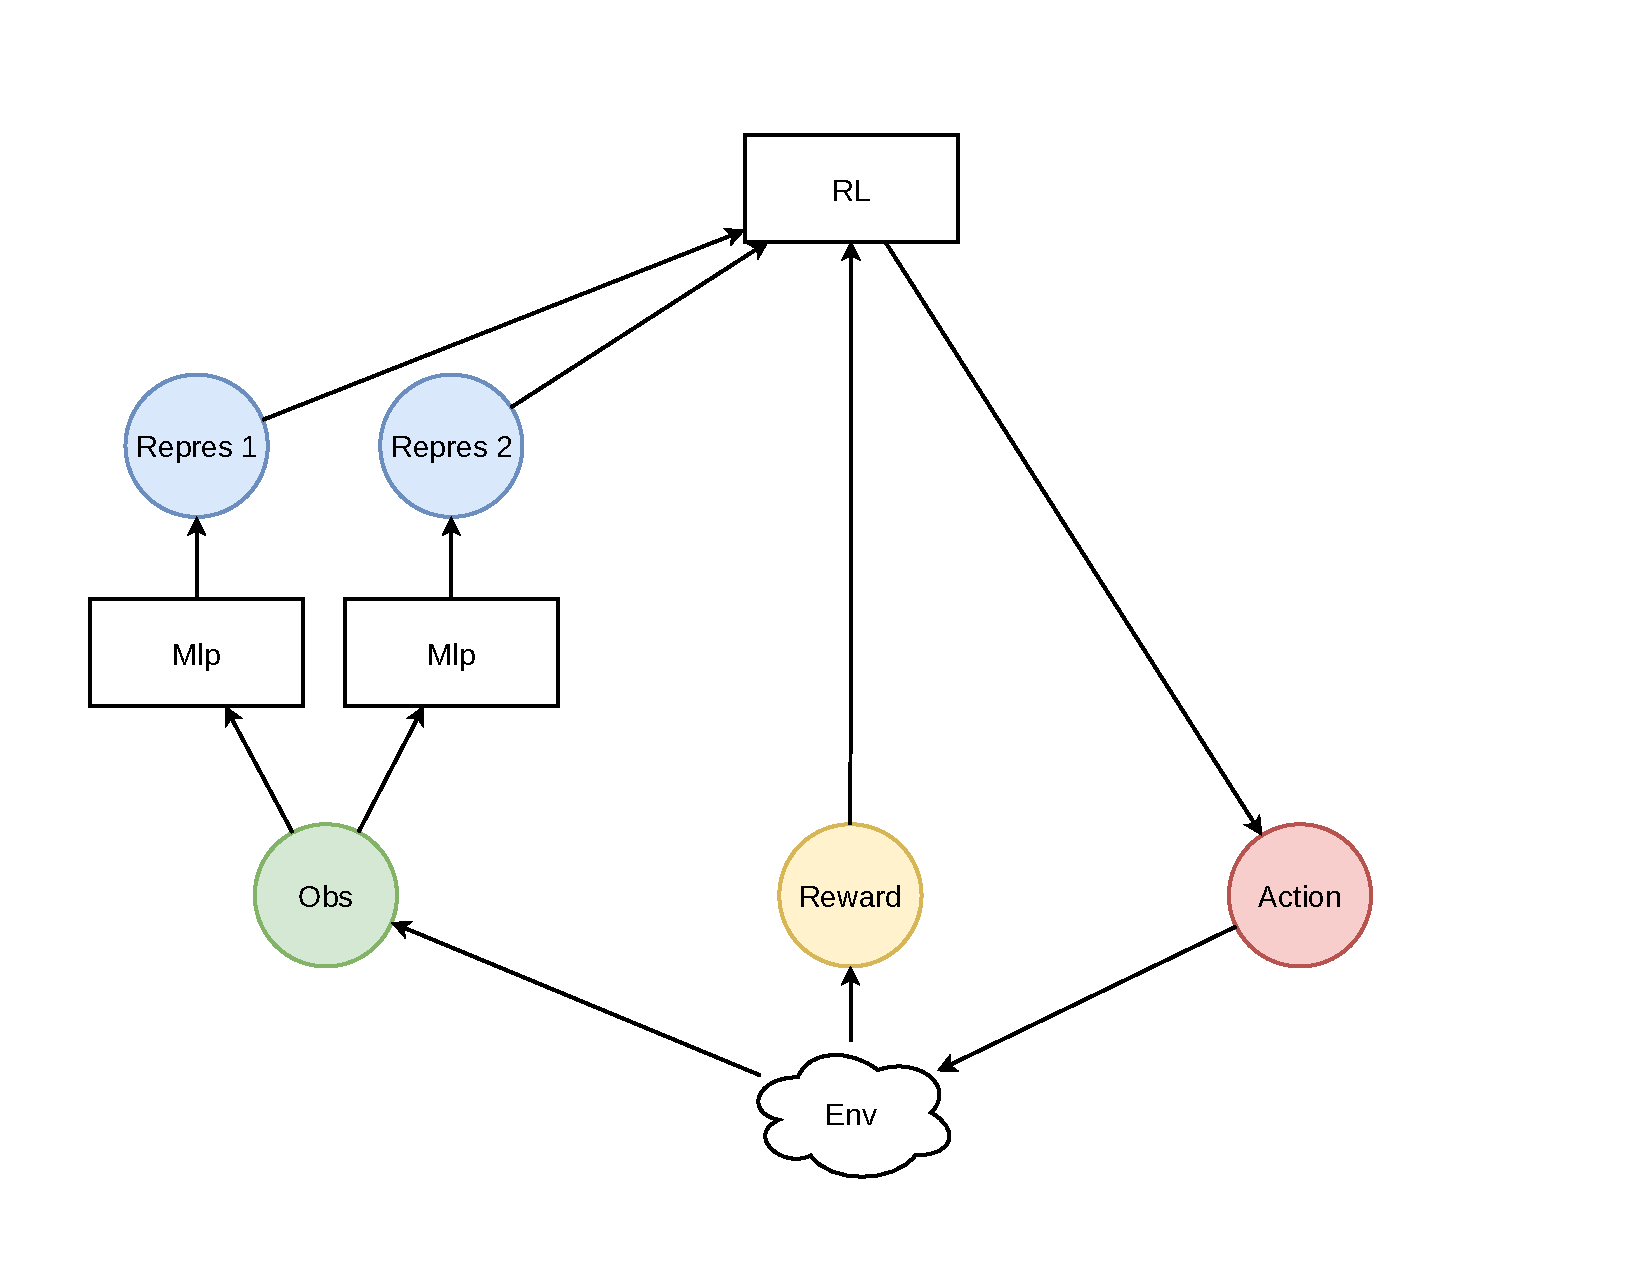
\includegraphics[width=0.8\textwidth]{images/step-0.pdf}
\end{figure}

This is a standard RL model, with two different MultiLayer Perceptron (MLP) modules.
The representation (in blue) will be aggregated into the RL core algorithm.

Later in this project, my job is to produce better representations for the RL core algorithm on the left side.
And in the future, maybe use modularized hierarchical RL on the right side.

I will probably start with something similar to the World Model \cite{ha_world_2018}, since it utilizes CNN, VAE, and RNN, which are all great tools.

Then, if possible, I'll do a Hierarchical version of the World Model maybe.

\subsubsection*{Environments}
My algorithm should be general, so it can work in different environments.

One possible testbed is the Continuous Control problem.
For example, locomotion is my most familiar task.

I also wish to test in some Card Games, so maybe I can ask my agent to play with someone else's agent.

\bibliographystyle{plain}
\bibliography{reference.bib}


\end{document}
